% --------------------------------------------------------------
% This is all preamble stuff that you don't have to worry about.
% Head down to where it says "Start here"
% --------------------------------------------------------------

\documentclass[11pt,oneside]{article}

\usepackage[margin=1in]{geometry} 
\usepackage[spanish]{babel} 
\usepackage{color}
\usepackage{rotating}
\usepackage{fancybox}
\usepackage{lscape}
\usepackage{makecell}
\usepackage{graphicx}
\usepackage{ltablex}
\usepackage{titling}

\usepackage{booktabs}
\usepackage{multirow}

\usepackage{subcaption}
\usepackage[space]{grffile}
\usepackage[font=footnotesize,labelformat=simple]{subcaption}
\usepackage{float}
\usepackage{adjustbox}
\usepackage{graphicx}
\usepackage{threeparttable}
\usepackage{caption}
\usepackage{subcaption}
\usepackage{graphicx}
\usepackage{hyperref}
\usepackage[font=singlespacing]{caption}
\usepackage{longtable}
% Configuración de los márgenes
\geometry{
	left=3cm, % Margen izquierdo de 3 cm
	right=3cm, % Margen derecho de 3 cm
	top=2.5cm, % Margen superior de 2.5 cm
	bottom=2.5cm % Margen inferior de 2.5 cm
}

\usepackage{parskip}

\usepackage{amsmath,amsthm,amssymb}
\newcommand{\code}{\texttt}
\newcommand{\N}{\mathbb{N}}
\newcommand{\Z}{\mathbb{Z}}
\newcommand{\E}{\mathbb{E}}


\newenvironment{theorem}[2][Theorem]{\begin{trivlist}
		\item[\hskip \labelsep {\bfseries #1}\hskip \labelsep {\bfseries #2.}]}{\end{trivlist}}
\newenvironment{lemma}[2][Lemma]{\begin{trivlist}
		\item[\hskip \labelsep {\bfseries #1}\hskip \labelsep {\bfseries #2.}]}{\end{trivlist}}
\newenvironment{exercise}[2][Exercise]{\begin{trivlist}
		\item[\hskip \labelsep {\bfseries #1}\hskip \labelsep {\bfseries #2.}]}{\end{trivlist}}
\newenvironment{problem}[2][Problem]{\begin{trivlist}
		\item[\hskip \labelsep {\bfseries #1}\hskip \labelsep {\bfseries #2.}]}{\end{trivlist}}
\newenvironment{question}[2][Question]{\begin{trivlist}
		\item[\hskip \labelsep {\bfseries #1}\hskip \labelsep {\bfseries #2.}]}{\end{trivlist}}
\newenvironment{corollary}[2][Corollary]{\begin{trivlist}
		\item[\hskip \labelsep {\bfseries #1}\hskip \labelsep {\bfseries #2.}]}{\end{trivlist}}

\newenvironment{solution}{\begin{proof}[Solution]}{\end{proof}}

% Load bibtex packages, including multibib to allow separate main paper \& appendix bibliographies.
\usepackage[round]{natbib}
\usepackage{authblk}
\usepackage{multibib}
\newcites{app}{Appendix References}


\begin{document}
	
% --------------------------------------------------------------
%                         Start here
% --------------------------------------------------------------
	
\title{Predicciones salariales en Colombia: \\
Un análisis utilizando la GEIH\thanks{Este trabajo corresponde al Trabajo Práctico 1 del curso de Machine Learning de la Maestría en Economía de la UNLP.}}

\vspace{2cm}

\author{
    Emiliano Bohorquez 

    Brayan A. Condori Luque}
	
\maketitle
	
\newpage
%%%%%%%%%%%%%%%%%%%%%%%%%%%%%%%%%%%%%%%%%%%%%%%%%%%%%%%%%%%%%%%%%%%%%%%%
% INTRODUCTION
%%%%%%%%%%%%%%%%%%%%%%%%%%%%%%%%%%%%%%%%%%%%%%%%%%%%%%%%%%%%%%%%%%%%%%%%

	\section{Introducción}

	La discusión sobre los ingresos laborales es relevante tanto para \textit{policymakers} como para economistas. Desde el punto de vista de las políticas públicas, su utilidad responda a la importancia de identificar a hogares vulnerables y mejorar el alcance de los programas sociales destinados a reducir las desigualdades de ingresos\footnote{Por ejemplo, en Perú, la pandemia evidenció la necesidad de contar con mejores estimaciones del ingreso per cápita, dado que esta variable se instrumentó como criterio de elegibilidad para programas de transferencias de emergencia}. Una medición errónea de los ingresos puede traducirse en sobreexclusión (o sobreinclusión) de participantes y, en consecuencia, reducir la efectividad de un programa. 

	Desde la perspectiva de las finanzas públicas, la subdeclaración de ingresos constituye uno de los principales desafíos para los gobiernos, ya que genera una reducción en los ingresos tributarios. En Estados Unidos, aproximadamente el 83,6\% de los impuestos se paga de manera voluntaria y puntual, lo cual genera un a brecha que puede atribuirse al subreporte \citep{tax}. Asimismo, la evasión de impuestos es un problema que dependiendo de quiénes y en qué magnitud, sus consecuencias van más allá de las cuentas fiscales, sino que también exacerba la desigualdad \citep{alstadsaeter2019tax}.
	
	La precisión en la predicción de los ingresos individuales importa para la investigación económica en general. Es común incluir estimaciones del ingreso laboral como regresores, sin embargo, si por se encuentran mal calculadas (subreporte en encuestas), las estimaciones podrían ser sesgadas. Se ha explorado ampliamente los errores de medición en los ingresos laborales, la tendencia es que hay sesgo de subreporte en los salarios (\citealp{moore2000income}; \citealp{bound2001measurement}). Por ello, resulta relevante predecir los ingresos individuales. 
	
	Utilizando datos de Bogotá provenientes de la Gran Encuesta Integrada de Hogares (GEIH) de 2018, construimos un modelo que predice los ingresos horarios individuales. Esta base de datos a nivel individual incluye información laboral y sociodemográfica clave para predecir los salarios.
	

	%%%%%%%%%%%%%%%%%%%%%%%%%%%%%%%%%%%%%%%%%%%%%%%%%%%%%%%%%%%%%%%%%%%%%%%%
	% PREGUNTA 2
	%%%%%%%%%%%%%%%%%%%%%%%%%%%%%%%%%%%%%%%%%%%%%%%%%%%%%%%%%%%%%%%%%%%%%%%%
	\section{Datos}
	
	El conjunto de datos utilizados proviene de la GEIH de Colombia para la ciudad de Bogotá, la cual tiene por finalidad brindar información socioeconómica y sobre la situación laboral del país a través de una muestra representativa de dicha población (DANE-DIMPE, 2023)\footnote{Para más información, véase el documento oficial de la DANE disponible en \href{https://ignaciomsarmiento.github.io/GEIH2018_sample/ddi-documentation-spanish-608.pdf}{este enlace}.}.

	
	Esta base es el insumo principal para nuestro modelo de predicción salarial, ya que cuenta con diferentes variables que representan la remuneración de un trabajador (ingreso laboral mensual, ingreso laboral mensual por hora, salario de ocupación principal, salario mensual por hora, entre otros). Además, contiene un conjunto de características claves que funcionan como predictoras tales como la edad, el género y el nivel educativo. Por otra parte, el número de observaciones utilizadas en este estudio es de 9844, lo que permite tener una muestra grande para posteriormente dividirla en conjunto de entrenamiento y conjunto de prueba. 
	
	El trabajo fue realizado en el lenguaje de programación Python dada su potencia y versatilidad para trabajar con grandes volúmenes de datos. A continuación, se detalla el proceso de obtención, limpieza, transformación y descripción de este insumo. 
	
	\subsection{Obtención de datos}
	
	La obtención de la base completa requirió la realización de un proceso de \textit{Web Scraping} del sitio web (\href{https://ignaciomsarmiento.github.io/GEIH2018_sample/}{GEIH DATA}). Específicamente se realiza un scrapeo horizontal, ya que se extrae información de diversas páginas. Cabe destacar que no se presentaron restricciones que dificultaran o imposibilitaran la obtención de datos\footnote{El repositorio de GitHub \href{https://github.com/ebqz7/Machine_Learning_TP}{TP1} contiene los \textit{scripts} que detallan el paso a paso.}. 
	
	\subsection{Limpieza y transformación de los datos}
	
	Para el análisis predictivo, restringimos la muestra bajo los siguientes criterios: (i) matoría de edad, y; (ii) que cuente con ingreso positivo. Se procedió a filtrar por la variable edad, lo que implicó eliminar de la base a todo aquel que no tenga 18 años. Por otra parte, se utilizó la variable de salario mensual por hora para quedarnos con todos aquellos que percibieran una remuneración. 
	
	Respecto a los \textit{missing values}, se decidió eliminar todo aquel dato faltante, quedándonos con 9.844 observaciones. Posteriormente realizamos una selección de columnas: el directorio del individuo, el identificador de hogar, el identificador de persona, el género, la edad, el estrato socioeconómico, si cuenta con empleo formal, el máximo nivel educativo, el ponderador de frecuencias, el salario horario mensual y el ingreso total mensual, que cumplirán un rol central en nuestro modelo. 
	
	Por otra parte, se llevó a cabo a una serie de transformaciones en algunas variables. En primer lugar, y que será de utilidad para el análisis descriptivo, se aplica logaritmo natural al salario mensual por hora para aproximar su distribución a una normal. Asimismo, observamos que la GEIH pregunta directamente si se percibe algún tipo de subsidio, los cuales pueden ser alimentario, en transporte, familiar o educativo. Por lo tanto, se procedió a generar una única variable dicotómica donde 1 representaría que un individuo sí percibió alguno de los auxilios mencionados antes, y 0 para el caso contrario.
	
	\subsection{Análisis descriptivo}
	
	Para culminar esta sección, realizamos un análisis descriptivo con los datos resultantes, el cual va desde cuadros con estadísticas relevantes hasta gráficos para observar la distribución del salario por hora. La tabla 1 realiza un resumen de la media, el desvío, el total de observaciones, y el mínimo y máximo valor. Cabe destacar el uso del ponderador "fweight" para que los datos sean representativos de la población.
	
	\begin{table}[H]
\caption{Estadísticas descriptivas del Salario por hora mensual}
		\centering
		\begin{tabular}{lccccc}
			\hline
			\textbf{Media} & \textbf{Desvío std} & \textbf{Población} & \textbf{Mínimo} & \textbf{Máximo} \\ \hline
			7.968,09 & 11.690,91 & 2.459.723 & 151,91 & 291.666,66 \\ \hline
		\end{tabular}
		\label{tab:estadisticas}
	\end{table}
	
	En primer lugar, el salario por hora promedio es de \$COL 7.968,09, con un desvío estándar de \$COL 11.690,91, para una población representada de 2.459.723. El valor mínimo en el rango es de \$COL 151,91 y el máximo es de \$COL 291.666.66. Estas estadísticas nos muestran que existe una dispersión importante en los datos, producto de valores extremos en la cola superior. Esto refuerza la convención que las distribuciones de ingresos (y salarios) presentan una asimetría negativa. El gráfico \ref{fig:graph} confirma nuestras apreciaciones.
	
	Para facilitar la interpretación del gráfico de densidad, utilizamos la variable logarítmica del salario por hora (véase gráfico \ref{fig:graph_1}).
	
	Tal como venimos mencionando, observamos que la curva tiene un sesgo hacia la derecha, indicando que la media es mayor que la mediana salarial producto de los valores en la cola superior. Evidenciamos un pico alrededor de un salario horario de \$COL 2.980, y una mayor dispersión entre este último y $ln(10)$ que es igual a \$COL 22.026, lo que indica que la mayoría de las observaciones se encuentran dentro de este rango. 
	
	Ahora bien, veamos cómo se modifican los estadísticos si desagregamos por un conjunto de variables. La tabla 2 resume esta información por género. 
	
	\begin{table}[H]
\caption{Estadísticas descriptivas por género}
        \centering
		\begin{tabular}{lccccc}
			\hline
			\textbf{Género} & \textbf{Media} & \textbf{Desvío std} & \textbf{Población} & \textbf{Mínimo} & \textbf{Máximo} \\ \hline
			Mujer & 7.808,22 & 10.903,69 & 1.211.179 & 151,91 & 175.000 \\ 
			Varón & 8.123,18 & 12.406,07 & 1.248.544 & 518,52 & 291.666,66 \\ \hline
		\end{tabular}
		\label{tab:estadisticas_genero}
	\end{table}
	
	Para el caso de las mujeres, el salario por hora medio es de \$COL 7.808,22, mientras que para los varones es de \$COL 8.123,18, es decir que en promedio el género masculino gana un 4\% que el femenino según la muestra trabajada. Sin embargo, la dispersión para los primeros es mayor que para estas últimas, como así también los valores mínimo y máximo. Por lo tanto, existe una brecha de género que la media no termina de capturar, pero que se demuestra en la variabilidad de estos datos. El gráfico \ref{fig:graph_2} ilustra la distribución por sexo utilizando el logaritmo del salario. 
	
	Como podemos observar, la curva de densidad para los varones presenta un grado mayor de dispersión que la equivalente para mujeres, además de tener un mayor sesgo hacia la derecha.
	
	Por otro lado, la tabla 3 muestra las estadísticas descriptivas dividido si la persona tiene un empleo formal, o dicho de otra manera, si cuenta con un registro en la seguridad social.
	
	\begin{table}[H]
        \centering
        \caption{Estadísticas descriptivas por registro laboral}
		\begin{tabular}{lccccc}
			\hline
			\textbf{Registro} & \textbf{Media} & \textbf{Desvío std} & \textbf{Población} & \textbf{Mínimo} & \textbf{Máximo} \\ \hline
			Formal   & 9.123,23 & 12.799,65 & 1.886.900 & 151,91 & 291.666,66 \\ 
			Informal & 4.163,04 & 5.327,54  & 572.823   & 326,67 & 136.111,11 \\ \hline
		\end{tabular}
		\label{tab:estadisticas_registro}
	\end{table}
	
	Un empleado formal tiene un salario horario medio que equivale a más de dos ingresos de los informales. Especificamente, la remuneración esta por encima en un 119\%. Sin embargo, hay una diferencia significativa entre el total de formales, 1.886.900, y el total de no formales, 572.823. Esto nos indica 2 cosas: (i) con los filtros realizados, capturamos una porción importante de los empleados registrados, pero no ocurre lo mismo con los no registrados en la seguridad social, y (ii) los informales pueden tener ingresos provenientes de otras ocupaciones, incluso más de una, por ende la variable de referencia seleccionada, el salario por hora mensual, no sería la adecuada para capturar este segmento de la población. El gráfico \ref{fig:graph_3} vislumbra la distribución de lo mencionado previamente. 
	
	Tomando el logaritmo natural del salario por hora mensual, los formales presentan un sesgo hacia la derecha, y los salarios están concentrada entre $ln(8)$ y $ln(10)$, mientras que para los no formales la dispersión es más alta, indicando una mayor heterogeneidad, y también cuentan con una asimetría positiva pero menos marcada.
	
	Por último, incorporamos al análisis dos gráficos más donde vemos la distribución del logaritmo del salario por hora mensual según el estrato socioeconómico y el máximo nivel educativo alcanzado. Tomando el primero, la GEIH define 6 grupos para el \textit{estrato socioeconómico} en función de la zona donde se encuentre la persona encuestada. Si esta reside en una de las 13 áreas metropolitanas, entonces se define su grupo social en función del consumo energético, mientras que, si vive en las cabeceras o en las zonas rurales, para la clasificación se utiliza el Índice de Calidad de Vida, integrando factores de bienestar vinculados a accesibilidad de servicios, condiciones de hábitat e ingresos (véase gráfico \ref{fig:graph_4}).
	
	En primer lugar, observamos mayor presencia de los 3 primeros estratos socioeconómicos, es decir, los más vulnerables. Estos grupos se encuentran concentrados alrededor de un salario horario mensual de \$COL 2.980, aunque el tercer sextil presenta una mayor dispersión. Por otra parte, los 3 sextiles superiores tienen un volumen de observaciones mucho menor, presentan una mayor duspersión en comparación a los estratos inferiores, y su moda esta alrededor de una remuneración por hora mensual de \$COL 22.026. 
	
	El gráfico \ref{fig:graph_5} ilustra la distribución salarial por máximo nivel educativo alcanzado. Las categorías van desde \textit{sin instrucción} hasta \textit{nivel superior}. Cabe destacar que, dado el filtrado de datos, el nivel faltante es \textit{preescolar completo}.
	
	Estas curvas de densidad tienen en común que todas tienen un pico en $ln(8)$ que es igual a \$COL 2.980. Sin embargo, para los niveles educativos más bajos la densidad es mucho más baja, mientras que es mayor para los dos niveles más altos, \textit{secundario completo y superior}. Este último, cuenta con una dispersión más alta que el resto, producto de la heterogeneidad de salarios entre personas con nivel superior, ya sea que este fuera completado o no. 
	
	En síntesis:
	\begin{enumerate}
		\item La muestra presenta importante variabilidad en los salarios por hora mensuales, además de contar con una asimetría positiva en la distribución.
		\item Existen diferencias por género no captadas en las medias salariales, pero sí en su dispersión.
		\item Con los filtros realizados y la variable de ingresos elegida captamos bien a los trabajadores formales, pero no así a los informales. Además, un trabajador formal tiene un salario por hora medio hasta dos veces más grande que un informal. 
		\item Los 3 sextiles inferiores tienen mayor presencia en el conjunto de datos y están más concentrados, mientras los 3 sextiles superiores están más dispersos y cuentan con menor volumen de observaciones. Estos últimos evidencian un salario mayor que los grupos más vulnerables.
		\item Secundario completo y nivel superior son los dos máximos niveles educativos con mayor densidad en la distribución. Respecto a todos los niveles, estos están concentrados alrededor del mismo punto, pero quienes cuentan con formación terciaria/universitaria presentan mayor heterogeneidad. 
	\end{enumerate}
	
	
	
	
	
	%%%%%%%%%%%%%%%%%%%%%%%%%%%%%%%%%%%%%%%%%%%%%%%%%%%%%%%%%%%%%%%%%%%%%%%%
	% PREGUNTA 3 
	%%%%%%%%%%%%%%%%%%%%%%%%%%%%%%%%%%%%%%%%%%%%%%%%%%%%%%%%%%%%%%%%%%%%%%%%
	\section{Predicción de los ingresos salariales}
	
	El modelo con el que buscamos predecir el salario por hora mensual es el siguiente:
	
	\begin{center}
		$w = f(X) + u$
	\end{center}
	
	Como ya mencionamos, $w$ es el salario por hora mensual que percibe un trabajador. $f(X)$ es el conjunto de predictores, donde las variables elegidas son: la edad, el género, si es trabajador formal, el estrato socioeconómico, el máximo nivel educativo y si percibe subsidio. Por último $u$ es un término error.
	
	En primer lugar, vamos a dividir aleatoriamente el conjunto de datos en dos: un conjunto de entrenamiento, que cumplirá la función de insumo para que el modelo aprenda de los datos y ajuste sus parámetros, y un conjunto de prueba, utilizado para evaluar la capacidad del modelo. Para el primero será asignado un 70\% de la muestra, y para el testing el 30\% restante.
	
	Segundo, estimamos el modelo a través de una iteración donde vamos agregando los predictores mencionados arriba. En total se corren 6 modelos lineales. La tabla 4 resume los resultados especificando el RMSE (raiz cuadrada del error cuadrático medio) tanto del conjunto de entrenamiento como del de prueba. Adicionalmente, se incorpora una columna llamada \textit{Error}, la cual se obtiene de dividir el RMSE de los datos de testing respecto de la media de la variable dependiente del mismo conjunto, permitiendo verificar cuánto la estimación se aleja de la media (expresado en porcentajes). 
	
	\begin{table}[H]
		\centering
        \caption{Performance predictiva de los modelos lineales}
		\begin{tabular}{lccccc}
			\hline
			\textbf{Modelo} & \textbf{Parámetros} & \textbf{RMSE (train)} & \textbf{RMSE (test)} & \textbf{Coef. Error} \\ \hline
			1 & 1 & 11508,82 & 11521,53 & 1,50 \\ 
			2 & 2 & 11506,43 & 11519,97 & 1,50 \\ 
			3 & 3 & 11300,71 & 11401,09 & 1,48 \\ 
			4 & 4 & 9877,09  & 10231,75 & 1,33 \\ 
			5 & 5 & 9743,66  & 10081,41 & 1,31 \\ 
			6 & 6 & 9485,92  & 9766,92  & 1,27 \\ \hline
		\end{tabular}
		\label{tab:modelos_rmse}
	\end{table}
	
	Partiendo de un modelo de regresión lineal simple, con la edad como único predictor, el RMSE en el entrenamiento es de 11.508,82 unidades frente a las 11.521,53 unidades del RMSE del testing. El coeficiente de error es de 1,5\%. Si vamos incorporando variables, observamos que los errores de ambos conjuntos se reducen hasta el último modelo lineal que cuenta con 6 predictores y tiene un RMSE de 9.485,92 para el conjunto de entrenamiento y de 9.766,92 para el conjunto de prueba, siendo el coeficiente de error de 1,27\%. 
	
	Adicionalmente, generamos una transformación polinómica en el modelo con todos las variables explicativas para encontrar una versión que alcance el RMSE mínimo en el conjunto de testing. Una simplificación de la ecuación sería la siguiente:
	
	\begin{center}
		$w = \beta_{1}X + \beta_{2}X^2 + ... + \beta_{p}X^p + u$
	\end{center}
	
	Los grados del polinomio se modificarán iterativamente iniciando por un grado 2 hasta un modelo con grado 6. La tabla 5 ilustra los resultados.
	
	\begin{table}[H]
		\centering
        \caption{Performance predictiva de los modelos polinómicos}
		\begin{tabular}{lccccc}
			\hline
			\textbf{Modelo} & \textbf{Parámetros} & \textbf{RMSE (train)} & \textbf{RMSE (test)} & \textbf{Coef. Error} \\ \hline
			7  & 28  & 8353,87  & 9133,29  & 1,19 \\ 
			8  & 84  & 7814,41  & 9228,33  & 1,20 \\ 
			9  & 210 & 7443,48  & 9525,96  & 1,24 \\ 
			10 & 462 & 7276,48  & 10200,02 & 1,33 \\ 
			11 & 924 & 7160,97  & 17569,97 & 2,29 \\ \hline
		\end{tabular}
		\label{tab:modelos_rmse}
	\end{table}
	
	Primero, evidenciamos que el número de parámetros se incrementa exponencialmente donde, por ejemplo, en el último modelo la cantidad de predictores se incrementa a 924. Sin embargo, aquí empiezan a divergir los RMSE de ambos conjuntos. Para el entrenamiento, la raíz del error cuadrático medio se reduce hasta tender a un valor levemente superior a las 7.000 unidades, mientras que en el testeo el RMSE disminuye en el modelo de grado 2, pero se incrementa a partir de la transformación de grado 3, teniendo un salto exponencial en el último de grado 6. Esto indica que al incrementar los predictores, el modelo incorpora el ruido del conjunto de datos, volviendo las predicciones más imprecisas.  
	El gráfico \ref{fig:graph_6} ilustra la complejidad de todos los modelos frente a la raíz del error cuadrático medio. 
	
	% AQUI VA GRAFICO 7
	
	Los modelos con mejor performance predictiva son el modelo 7, que tiene un grado polinómico igual a 2, y el modelo 8, con un grado polinómico igual a 3. Ambos tienen los menores RMSE con 9.133,29 y 9.228,33 unidades, respectivamente. Además, el coeficiente de error es de 1,19\% para el primero, y 1,20\% para el segundo, permitiendonos concluir que la relación entre una serie de predictores basados en características personales y socioeconómicas, junto sus respectivas interacciones, se relacionan de forma no-lineal con el salario por hora mensual. 
	
	\subsection{Errores de Predicción}

    Analizamos los errores de predicción de los modelos con mejor performance. El gráfico \ref{fig:3c3_boxplot} muestra el diagrama de caja para ambos modelos\footnote{ El análisis es análogo para la variable en su versión logarítimica. Ver gráfico \ref{fig:3c3_boxplot_log}.}. En ambos casos, el rango intercuantil (25,75) está centrado en cero, lo que indica su gran capacidad predictiva y que no existe un sesgo sistemático. Los outliers en ambos casos representan menos del 0.5\% del total de la muestra\footnote{Existen 37 y 42 outliers para los modelos 7 y 8, respectivamente. Se calcula el z-score y se considera outlier si la observación se ubica más de tres desviaciones estándar de la media.}, por lo que su presencia, aunque reduce el poder predictivo del modelo no representa una seria amenaza al poder de predicción a menos que sea sistemático en grupos específicos de personas.

    Estos outliers, al representar un proporción reducida de la muestra, pueden ser objetivo de análisis minucioso por parte de la DIAN. Dada la gran capacidad predictiva de ambos modelos, no resulta sensato pensar que los outliers puedan ser consecuencia de una incorrecta especificación del modelo.

	\subsection{Método Leave-One-Out Cross Validation (LOOCV)}
	
	Usando los modelos con menor error predictivo calculados mediante el \textit{validation set approach}, calculamos nuevamente el RMSE mediante el método LOOCV. Este método lleva al extremo el mñetodo usado previamente al crear tantos grupos de entrenamiento y muestra como observaciones, donde se usa cada observación como conjunto de prueba y el resto como conjunto de entrenamiento.

    Utilizando los modelos con menor error predictivo, calculados mediante el \textit{validation set approach}, calculamos nuevamente el RMSE utilizando el método LOOCV. Este enfoque lleva al extremo el método previamente aplicado, ya que crea tantos conjuntos de entrenamiento y prueba como observaciones existen en la muestra. En cada iteración, se emplea una observación como conjunto de prueba, mientras que el resto se utiliza para el entrenamiento.




La tabla \ref{tab:comparacion} resume el calculo de los errores de predicción bajo tres métodos: validation set, LOOCV y K-Fold. 

	\begin{table}[H]
		\centering
        \caption{Performance predictiva de los modelos polinómicos}
		\begin{tabular}{lccc}
            \hline
            \textbf{Modelo} & \textbf{RMSE (testing)} & \textbf{RMSE (LOOCV)} & \textbf{RMSE (KFold)} \\ \hline
            Modelo 7        & 9133.29                & 3770.06               & 8492.59               \\
            Modelo 8        & 9228.33                & 3471.45               & 8190.87               \\ \hline
    \end{tabular}
		\label{tab:comparacion}
	\end{table}


Existe una discrepancia en los resultados. Mientras que el \textit{validation set approach} sugiere que el modelo 7 tiene un mejor desempeño, el metodo LOOVC favorece al modelo 8. Esta diferencia puede atribuirse a tres razones:
\begin{itemize}
    \item \textbf{Sesgo de muestra en el \textit{validation set approach}:} La selección de amos grupos se realiza de manera aleatoria. Esto puede crear conjuntos de entrenamiento y de prueba que no representan la distribución de los datos. 
    \item \textbf{Senbilidad del método LOOCV a outliers:} El método es sensible a outliers por construcción, dado que cada observación, incluyendo los extremos, forman parte del conjunto de prueba.
    \item \textbf{Complejidad del modelo:} El polinomio de grado 3 (modelo 8) muestra una mejor generalización sobre multiples conjuntos de entrenamiento, como sucede con el método LOOCV. Sin embargo, ello no garantiza que su desempeño sea el óptimo para todas las configuraciones de muestras.
\end{itemize}


Por ello, calculamos el error de predicción usando el método K-Fold\footnote{Se utiliza un \code{random state = 123} y 10 submuestras.}. Este método, similar a LOOCV, utiliza submuestras en lugar de observaciones individuales como unidad de iteración. Bajo este método, el modelo con menor error de predicción es el modelo 8.

\newpage

\section{Conclusión}

La predicción de los salarios individuales es relevante para objetivos de política pública. Haciendo uso de la GEIH de Colombia para la ciudad de Bogotá, proponemos un modelo predictivo de los salarios horarios. Las variables incluidas como predictores se basan en características personales y socioeconómicas. Para el primer grupo, se incluyen la edad y el género; y para el segundo, el estrato social, la situación laboral respecto a si esta registrado o no, el máximo nivel educativo alcanzado y si percibe algún subsidio. 

Primeramente, se corrieron seis modelos lineales, a los cuales se les iba incorporando iterativamente las variables mencionadas previamente. Luego, se procedió a realizar transformaciones polinómicas, incrementando el grado de los modelos con todos los predictores. Los modelos con mejor performance predictiva, es decir aquellos con el menor error cuadrático medio, fueron el modelo con un grado polinómico igual a 2 e igual a 3, ambos con un coeficiente de error, respecto a la media del salario del conjunto de prueba, de 1,19\% y 1,20\%, respectivamente. Esto último nos permite afirmar que la relación entre las variables predictoras y el salario por hora mensual es no lineal. 

Para estos dos modelos, se analizó sus errores de predicción. Ambos modelos tienen un buen desempeño, dado que la masa de la distribución está centrada en cero. La presencia de outliers en el error de predicción no supone un problema para el modelo, dado que representa menos del 0.5\% de la muestra; sin embargo, resulta relevante para decisiones de política, por ejemplo, la agencia tributaria podría auditar a estos individuos.

Finalmente, como análisis de robustez para la elección del mejor modelo predictivo, se calcula el RMSE mediante LOOCV y K-Fold. El modelo con mejor desempeño bajo distintas submuestras es el modelo polinómico de grado 3. 


	% --------------------------------------------------------------
	%     You don't have to mess with anything below this line.
	% --------------------------------------------------------------
	\newpage
	\bibliographystyle{ecta}
	\bibliography{references.bib}
	
	\newpage
	\appendix
	\setcounter{table}{0}
	\renewcommand{\tablename}{Cuadro}
	\renewcommand{\figurename}{Figura}
	\renewcommand{\thetable}{A\arabic{table}}
	\setcounter{figure}{0}
	\renewcommand{\thefigure}{A\arabic{figure}}
	%%%%%%%%%%%%%%%%%%%%%%%%%%%%%%%%%%%%%%%%%%%%%%%%%

\section{Anexos}

%-------------------------------------------------------------%
% GRÁFICO 1
\begin{figure}[H]
    \centering
    \caption{Distribución de los salarios por hora mensuales}
    \label{fig:graph}
        \includegraphics[width=0.8\textwidth]{images/graph.png} \\
\end{figure}


%-------------------------------------------------------------%
%-------------------------------------------------------------%
% GRÁFICO 2
\begin{figure}[H]
    \centering
    \caption{Distribución de los salarios por hora mensuales}
    \label{fig:graph_1}
        \includegraphics[width=0.8\textwidth]{images/graph_1.png} \\
\end{figure}


%-------------------------------------------------------------%
% GRAFICO 3
\begin{figure}[H]
    \centering
    \caption{Distribución de los salarios por hora mensuales - Por género}
    \label{fig:graph_2}
        \includegraphics[width=0.8\textwidth]{images/graph_2.png} \\
\end{figure}



%-------------------------------------------------------------%
%-------------------------------------------------------------%
% GRÁFICO 4
\begin{figure}[H]
    \centering
    \caption{Distribución de los salarios por hora mensuales - Por registro laboral}
    \label{fig:graph_3}
        \includegraphics[width=0.8\textwidth]{images/graph_3.png} \\
\end{figure}


%-------------------------------------------------------------%
% GRAFICO 5
\begin{figure}[H]
    \centering
    \caption{Distribución de los salarios por hora mensuales - Por estrato}
    \label{fig:graph_4}
        \includegraphics[width=0.8\textwidth]{images/graph_4.png} \\
\end{figure}



%-------------------------------------------------------------%
%-------------------------------------------------------------%
% GRÁFICO 6
\begin{figure}[H]
    \centering
    \caption{Distribución de los salarios por hora mensuales - Por máximo nivel educativo}
    \label{fig:graph_5}
        \includegraphics[width=0.8\textwidth]{images/graph_5.png} \\
\end{figure}


%-------------------------------------------------------------%
% GRAFICO 7
\begin{figure}[H]
    \centering
    \caption{Complejidad del modelo vs Error de predicción por conjunto}
    \label{fig:graph_6}
        \includegraphics[width=0.8\textwidth]{images/graph_6.png} \\
\end{figure}



%-------------------------------------------------------------%

% 3c3
\begin{figure}[H]
    \centering
    \caption{Box Plot de los errores de predicción de los modelos 7 y 8}
    \label{fig:3c3_boxplot}
        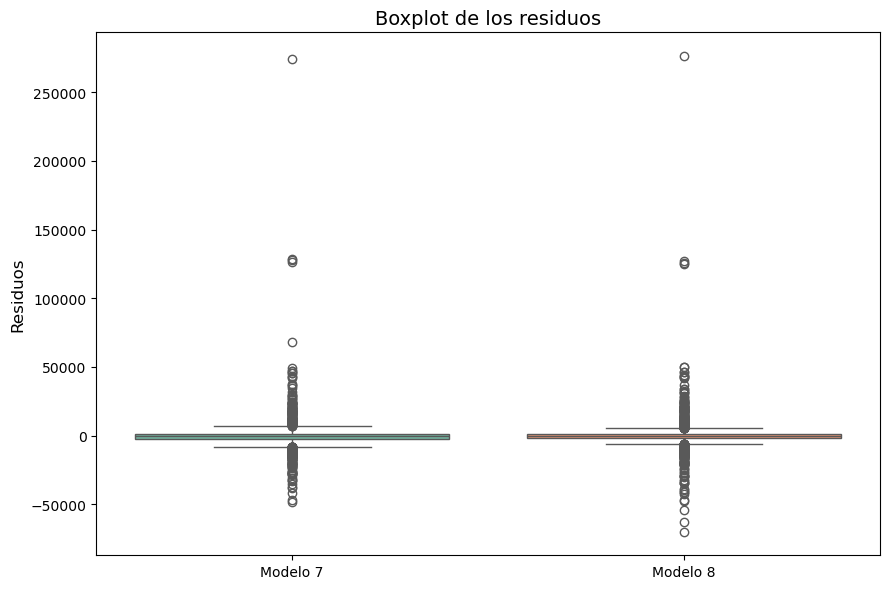
\includegraphics[width=0.8\textwidth]{images/boxplot_wage.png} \\
\end{figure}
%-------------------------------------------------------------%
%-------------------------------------------------------------%
% 3c3
\begin{figure}[H]
    \centering
    \caption{Box Plot de los errores de predicción de los modelos 7 y 8 (log)}
    \label{fig:3c3_boxplot_log}
        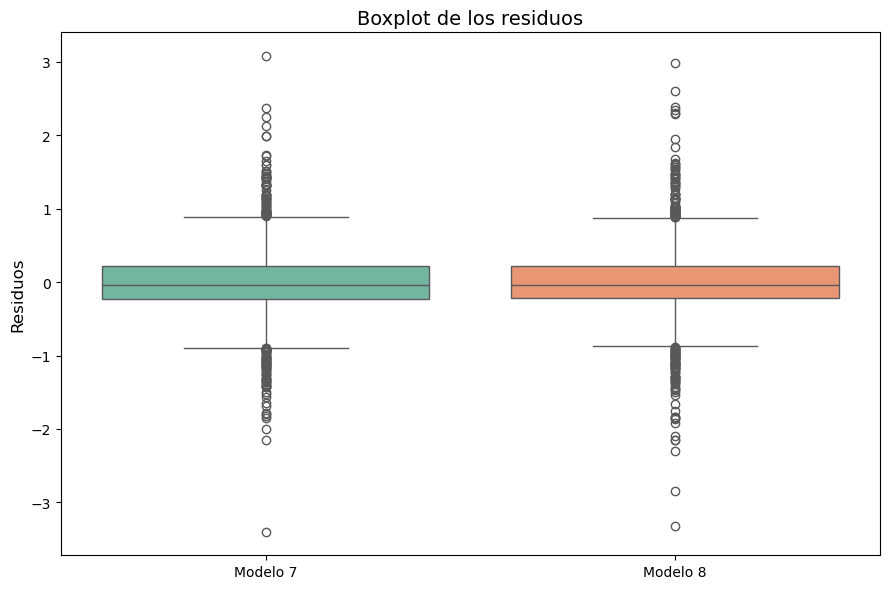
\includegraphics[width=0.8\textwidth]{images/boxplot_lnwage.png} \\
\end{figure}
%-------------------------------------------------------------%



\end{document}

